% =========================================================================
% System teaser -- TikZ, built with OpenTikZ
%   Left   : live speech into a small local full-duplex model
%   Centre : a probe taps a MID layer and decides in 20-45 ms, with a
%            conceptual timeline (end of turn -> probe -> first spoken word)
%   Right  : easy -> local answer;  hard -> cloud expert, returned through
%            the SAME local talker
%   Foot   : four icon cues (mid-layer probe / before speaking /
%            selective handoff / same session)
%
% The probe is the visual focus: it is the only saturated orange object and
% the only one with a halo. Aspect ~2.3:1 so the figure scales to ~0.70 at
% \linewidth and the smallest label stays above 5.5pt.
% Build: tectonic -X compile teaser_system.tex
% =========================================================================
\documentclass[border=8pt]{standalone}

\usepackage[T1]{fontenc}
\usepackage{lmodern}
\usepackage{tikz}
\usetikzlibrary{positioning, arrows.meta, decorations.pathreplacing, calc}

% --- OpenTikZ palette (light / default, color-blind-friendly Okabe-Ito) ---
\definecolor{otblue}{HTML}{0072B2}
\definecolor{otorange}{HTML}{E69F00}
\definecolor{otteal}{HTML}{009E73}
\definecolor{otpurple}{HTML}{CC79A7}
\definecolor{otgray}{HTML}{5A5A5A}

% ---- glyphs (adapted from OpenTikZ icons) -------------------------------
% person (icons/systems/user); base at (#1,#2), scale #3, colour #4
\newcommand{\otuser}[4]{%
  \begin{scope}[shift={(#1,#2)}, scale=#3, line width=1.1pt]
    \filldraw[draw=#4!75!black, fill=#4!18] (0,1.30) circle[radius=0.45];
    \filldraw[draw=#4!75!black, fill=#4!18]
      (-0.95,0) .. controls (-0.95,0.58) and (-0.55,0.80) .. (0,0.80)
      .. controls (0.55,0.80) and (0.95,0.58) .. (0.95,0) -- cycle;
  \end{scope}}

% cloud (icons/systems/cloud); anchored near (#1,#2), scale #3, colour #4
\newcommand{\otcloud}[4]{%
  \begin{scope}[shift={(#1,#2)}, scale=#3]
    \begin{scope}
      \clip (-1.55,-0.45) rectangle (1.9,1.35);
      \fill[#4, rounded corners=0.4cm] (-1.25,-0.45) rectangle (1.7,0.35);
      \fill[#4] (-0.8,0.02) circle[radius=0.5];
      \fill[#4] (-0.1,0.42) circle[radius=0.55];
      \fill[#4] (0.65,0.18) circle[radius=0.72];
      \fill[#4] (1.25,-0.04) circle[radius=0.46];
    \end{scope}
  \end{scope}}

% loudspeaker at (#1,#2), scale #3, colour #4
\newcommand{\otspeaker}[4]{%
  \begin{scope}[shift={(#1,#2)}, scale=#3]
    \filldraw[draw=#4!75!black, fill=#4!18, line width=1.1pt, line join=round]
      (-0.46,-0.20) -- (-0.16,-0.20) -- (0.20,-0.50) -- (0.20,0.50)
      -- (-0.16,0.20) -- (-0.46,0.20) -- cycle;
    \foreach \r in {0.24,0.44}{
      \draw[#4!75!black, line width=1.1pt, line cap=round]
        (0.28,0) ++(-45:\r) arc[start angle=-45, end angle=45, radius=\r];}
  \end{scope}}

% speech waveform: 9 bars starting at x=#1, centred on y=#2, colour #3
\newcommand{\otwave}[3]{%
  \foreach \i/\h in {0/0.20,1/0.44,2/0.30,3/0.62,4/0.80,5/0.52,6/0.70,7/0.34,8/0.18}{
    \draw[#3, line width=2.2pt, line cap=round]
      ({#1+\i*0.20},{#2-\h}) -- ({#1+\i*0.20},{#2+\h});}}

% THE PROBE (visual focus): #1=x, #2=tip y, #3=head bottom y, #4=head top y
\newcommand{\otprobe}[4]{%
  \fill[otorange!10]  (#1,#2) circle[radius=0.52];
  \fill[otorange!20]  (#1,#2) circle[radius=0.34];
  \fill[otorange!42]  (#1,#2) circle[radius=0.18];
  \draw[otorange!70!black, line width=2.2pt] (#1,#2+0.34) -- (#1,#3);
  \filldraw[draw=otorange!70!black, fill=otorange!80, line join=round, line width=0.8pt]
    (#1-0.15,#2+0.38) -- (#1+0.15,#2+0.38) -- (#1,#2) -- cycle;
  \filldraw[draw=otorange!70!black, fill=otorange!35, line width=1.3pt, rounded corners=4pt]
    (#1-0.42,#3) rectangle (#1+0.42,#4);
  % sensor eye in the head -- echoes the "mid-layer probe" cue in the footer
  \draw[otorange!70!black, line width=1.1pt] (#1,{(#3+#4)/2}) circle[radius=0.15];
  \fill[otorange!70!black] (#1,{(#3+#4)/2}) circle[radius=0.055];}

% --- footer cue icons: (x, y, colour) ------------------------------------
\newcommand{\oticoncross}[3]{%
  \draw[#3, line width=1.2pt] (#1,#2) circle[radius=0.23];
  \fill[#3] (#1,#2) circle[radius=0.07];
  \foreach \a in {0,90,180,270}{
    \draw[#3, line width=1.2pt, line cap=round] (#1,#2) ++(\a:0.29) -- ++(\a:0.13);}}

\newcommand{\oticonclock}[3]{%
  \draw[#3, line width=1.3pt] (#1,#2) circle[radius=0.27];
  \draw[#3, line width=1.3pt, line cap=round] (#1,#2) -- ++(90:0.16);
  \draw[#3, line width=1.3pt, line cap=round] (#1,#2) -- ++(0:0.20);}

\newcommand{\oticonfork}[3]{%
  \draw[#3, line width=1.3pt, line cap=round] (#1-0.30,#2) -- (#1-0.02,#2);
  \draw[#3, line width=1.3pt, line cap=round] (#1-0.02,#2) -- (#1+0.20,#2+0.21);
  \draw[#3, line width=1.3pt, line cap=round] (#1-0.02,#2) -- (#1+0.20,#2-0.21);
  \fill[#3] (#1+0.28,#2+0.25) circle[radius=0.07];
  \fill[#3] (#1+0.28,#2-0.25) circle[radius=0.07];}

\newcommand{\oticonloop}[3]{%
  \draw[#3, line width=1.3pt, -{Stealth[length=1.8mm]}, line cap=round]
    (#1,#2) ++(-35:0.27) arc[start angle=-35, end angle=255, radius=0.27];}

\begin{document}
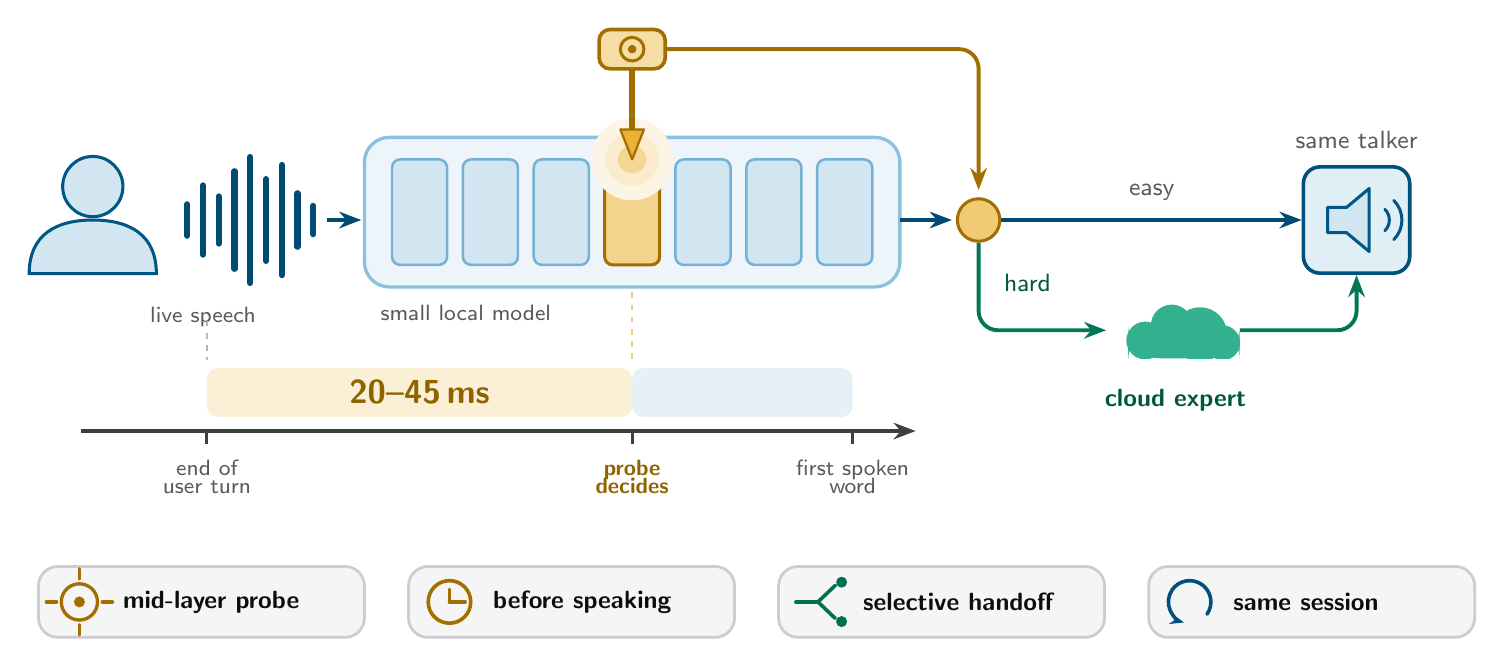
\begin{tikzpicture}[
    >={Stealth[length=2.8mm]},
    font=\sffamily,
    % ---- shared styles ---------------------------------------------------
    shell/.style={draw=otblue!45, fill=otblue!7, line width=1.2pt,
                  rounded corners=9pt},
    lay/.style={draw=otblue!55, fill=otblue!18, line width=0.9pt,
                rounded corners=3pt},
    layhi/.style={draw=otorange!70!black, fill=otorange!45, line width=1.1pt,
                  rounded corners=3pt},
    talker/.style={draw=otblue!70!black, fill=otblue!12, line width=1.3pt,
                   rounded corners=6pt, inner sep=0pt},
    pill/.style={draw=otgray!30, fill=otgray!6, line width=1pt,
                 rounded corners=7pt, inner sep=0pt},
    cue/.style={font=\sffamily\bfseries\small, text=otgray!15!black, anchor=west},
    lbl/.style={font=\sffamily\small, text=otgray},
    tny/.style={font=\sffamily\footnotesize, text=otgray, align=center},
    flow/.style={->, draw=otblue!65!black, line width=1.4pt},
    esc/.style={->, draw=otteal!75!black, line width=1.4pt},
    tap/.style={->, draw=otorange!70!black, line width=1.4pt},
    tie/.style={draw=otgray!45, line width=0.9pt, dash pattern=on 2pt off 2.4pt},
  ]

% =========================================================================
% LEFT -- live speech in
% =========================================================================
\otuser{1.15}{5.72}{0.85}{otblue}
\otwave{2.35}{6.40}{otblue!65!black}
\draw[flow] (4.12,6.40) -- (4.56,6.40);
\node[tny, anchor=north] at (2.55,5.42) {live speech};

% =========================================================================
% CENTRE -- the local model, tapped mid-stack by the probe
% =========================================================================
\draw[shell] (4.60,5.55) rectangle (11.40,7.45);
\foreach \i in {0,...,6}{
  \pgfmathsetmacro{\bx}{4.95+\i*0.90}
  \ifnum\i=3
    \draw[layhi] (\bx,5.83) rectangle (\bx+0.70,7.17);
  \else
    \draw[lay]   (\bx,5.83) rectangle (\bx+0.70,7.17);
  \fi}
\node[tny, anchor=north west] at (4.68,5.44) {small local model};

% the probe: tip on the middle layer, head above, wire out to the fork
\otprobe{8.00}{7.17}{8.32}{8.82}
\draw[tap, rounded corners=7pt] (8.42,8.57) -- (12.40,8.57) -- (12.40,6.78);

% -------- conceptual timeline (end of turn -> probe -> first word) --------
\def\ax{3.72}
\draw[->, draw=otgray!70!black, line width=1.2pt] (1.00,\ax) -- (11.60,\ax);
\foreach \t in {2.60,8.00,10.80}{
  \draw[draw=otgray!70!black, line width=1.1pt] (\t,\ax) -- (\t,\ax-0.17);}

% the pre-speech window: probe latency (orange) then remaining head-room
\fill[otorange!16, rounded corners=4pt] (2.60,3.90) rectangle (8.00,4.52);
\fill[otblue!10,   rounded corners=4pt] (8.00,3.90) rectangle (10.80,4.52);
\node[font=\sffamily\bfseries\large, text=otorange!62!black] at (5.30,4.21)
  {20--45\,ms};

% tie the timeline to what is happening above it
\draw[tie] (2.60,5.12) -- (2.60,4.62);
\draw[tie, draw=otorange!55] (8.00,5.48) -- (8.00,4.62);

\node[tny, anchor=north] at (2.60,\ax-0.24) {end of\\[-3pt]user turn};
\node[font=\sffamily\bfseries\footnotesize, text=otorange!62!black,
      anchor=north, align=center] at (8.00,\ax-0.24) {probe\\[-3pt]decides};
\node[tny, anchor=north] at (10.80,\ax-0.24) {first spoken\\[-3pt]word};

% =========================================================================
% RIGHT -- two paths, rejoining at the same talker
% =========================================================================
\draw[flow] (11.40,6.40) -- (12.06,6.40);
\filldraw[draw=otorange!70!black, fill=otorange!55, line width=1.1pt]
  (12.40,6.40) circle[radius=0.27];

\node[talker] (talk) at (17.20,6.40) [minimum width=1.35cm, minimum height=1.35cm] {};
\otspeaker{17.20}{6.40}{0.80}{otblue}
\node[lbl, anchor=south, align=center] at (17.20,7.18) {same talker};

% easy -> straight through, the local model answers
\draw[flow] (12.69,6.40) -- (talk.west);
\node[lbl, anchor=south] at (14.60,6.52) {easy};

% hard -> cloud expert, then back into the same talker
\draw[esc, rounded corners=7pt] (12.40,6.11) -- (12.40,5.00) -- (14.02,5.00);
\node[lbl, anchor=west, text=otteal!55!black] at (12.60,5.60) {hard};
\otcloud{14.90}{4.86}{0.48}{otteal!80}
\node[font=\sffamily\bfseries\small, text=otteal!55!black, anchor=north]
  at (14.90,4.38) {cloud expert};
\draw[esc, rounded corners=7pt] (15.72,5.00) -- (17.20,5.00) -- (talk.south);

% =========================================================================
% FOOT -- four icon cues
% =========================================================================
\foreach \cx/\txt in {2.53/{mid-layer probe}, 7.23/{before speaking},
                      11.93/{selective handoff}, 16.63/{same session}}{
  \draw[pill] (\cx-2.07,1.10) rectangle (\cx+2.07,2.00);
  \node[cue] at (\cx-1.12,1.55) {\txt};}
\oticoncross{0.98}{1.55}{otorange!70!black}
\oticonclock{5.68}{1.55}{otorange!70!black}
\oticonfork{10.38}{1.55}{otteal!70!black}
\oticonloop{15.08}{1.55}{otblue!70!black}

\end{tikzpicture}
\end{document}
